%%%%%%%%%%%%%%%%%%%%%%%%%%%%%%%%%%%%%%%%%%%%%%%%%%%%%%%%%%%%%%%%%%%%
%% estado_da_arte.tex
%% UNL thesis document file
%%%%%%%%%%%%%%%%%%%%%%%%%%%%%%%%%%%%%%%%%%%%%%%%%%%%%%%%%%%%%%%%%%%%
\chapter{Estado da arte}
\label{cha:estado_da_arte}

\section{Principais metodologias} % (fold)
\label{sec:principais_metodologias}

Para que esta dissertação pudesse apresentar vantagens em relação a trabalhos já desenvolvidos, foi necessário fazer uma pesquisa sobre as metodologias propostas para a solução ou diminuição de irregularidades existentes no asfalto, sendo que foram apenas encontrados trabalhos que propõem a deteção de buracos no asfalto, deixando de parte outras irregularidades como juntas de dilatação ou lombas. 
Após a análise de vários trabalhos relacionados com este problema, foi possível agrupar os trabalhos mais relevantes em categorias referentes às metodologias utilizadas para possíveis soluções, sendo os principais:
\begin{enumerate}
	\item \textbf{Câmera vídeo}
	\item \textbf{Câmera vídeo com iluminação artificial}
	\item \textbf{Ultrassom}
	\item \textbf{Acelerómetro}
\end{enumerate}
Nesta secção serão descritos os trabalhos e as tecnologias utilizadas em cada um deles, bem como as vantagens e desvantagens de cada uma das implementações apresentadas.

\subsection{Camera vídeo}
\label{subsec: camera_video}
No que toca às câmeras de vídeo, os trabalhos aqui referidos não são diretamente comparáveis com aquele que foi desenvolvido e é aqui apresentado, uma vez que utiliza uma tecnologia para a deteção e reconhecimento de buracos no asfalto bastante diferente da que foi utilizada nesta dissertação.
Ainda assim são trabalhos que se enquadram no tema e dos quais foram retiradas ideias para metodologias de comunicação entre os vários componentes da montagem.
De todos artigos estudados, três são aqueles que mostram abordagens mais interessantes, pois apresentam soluções diferentes entre si.
Em \cite{Zhang} e \cite{Chan2014} são utilizadas duas câmeras e apresentados algoritmos muito semelhantes, com resultados bastante positivos, sendo possível determinar uma relação entre estes trabalhos devido às várias colaborações já existentes entre os autores.
A solução proposta em \cite{Zhang} utiliza duas câmeras para criar uma imagem a três dimensões de modo a conseguir detetar um buraco no asfalto mas também calcular a sua profundidade.
Cruzando a imagem de ambas as câmeras, é possível encontrar os pontos comuns no asfalto de modo a sobrepor as imagens para o cálculo do desvio que existe entre elas de forma a criar um mapa virtual da superfície e do buraco.
Depois da criação do mapa é possível determinar qual o plano da estrada e também os pontos que se encontram abaixo desse plano, onde se encontram localizados os buracos.
O sistema é bastante preciso, permitindo a deteção de buracos com profundidades maiores que 4cm mas apresenta problemas de transmissão em tempo real uma vez que é necessário bastante processamento para fazer a sobreposição das imagens e também o mapeamento da superfície.

\begin{figure}[htbp]
	\centering
	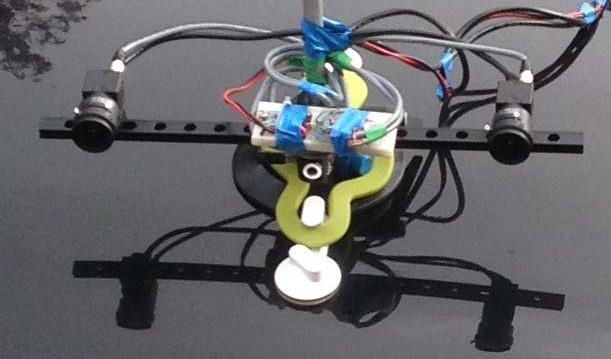
\includegraphics[height=6cm]{duas_cameras}
	\caption{Montagem com duas câmeras}
	\label{fig:montagem_com_duas_cameras}
\end{figure}

Em \cite{Chan2014} é apresentada uma melhoria a este sistema, no que toca ao processamento em tempo real, sendo que foram possíveis avaliar cinco imagens por segundo, uma a cada 200 milissegundos.
Juntando estes dois projetos é possível obter-se uma solução viável em termos de processamento e deteção mas que necessita de duas câmeras e um processador com vários núcleos para todo o processamento, tornando assim a sua montagem bastante dispendiosa.

Numa solução diferente, em \cite{Moazzam2013} é descrito um processo de deteção de buracos utilizando um sensor Kinect \footnote{https://developer.microsoft.com/en-us/windows/kinect} que só tem uma câmera mas tem um sensor de infravermelhos para determinar a distância a que se encontra de um objeto.
O sensor Kinect calcula a distância até um obstáculo e faz o mapeamento dessas distâncias, criando um mapa virtual do solo.
De seguida, as coordenadas X e Y do mapa são convertidas para o mundo real, de modo a obter as coordenadas reais.
São então feitos diversos cálculos para determinar as áreas de diferentes profundidades do buraco para que seja possível saber o volume que o buraco ocupa no asfalto.
Por fim os buracos são classificados com base nas curvas de relação área-profundidade, área ao nível do asfalto e profundidade máxima
Esta solução tem resultados semelhantes aos de \cite{Zhang} e \cite{Chan2014} e para a sua implementação são necessários menos cálculos, uma vez que o software Kinect está otimizado.
Além disso, embora não seja apresentado, é de esperar que esta opção seja menos dispendiosa que as anteriores graças ao preço do Kinect e que não seja necessário um processador tão potente.
Ainda assim existe a grande desvantagem do sistema só ter sido testado de forma imóvel, não existindo dados para a instalação em automóvel.

\begin{figure}[htbp]
	\centering
	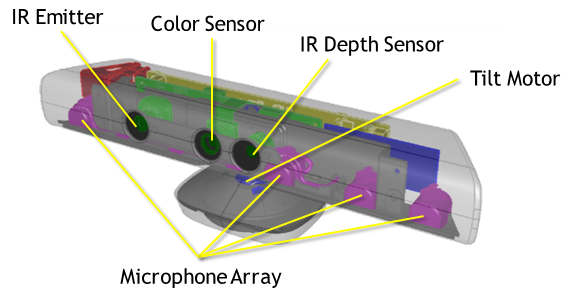
\includegraphics[height=5cm]{kinect}
	\caption[Sensor Kinect]{Sensor Kinect \footnotemark}
	\label{fig:sensor_kinect}
\end{figure}

\footnotetext{https://developer.microsoft.com/en-us/windows/kinect}

\subsection{Camera vídeo com iluminação artificial}
\label{subsec: camera_video_com_iluminacao_artificial}
Apesar dos artigos apresentados nesta secção utilizarem também câmeras, é interessante separá-los dos anteriores uma vez que a deteção dos buracos é feita de forma diferente, consoante a passagem pelo próprio buraco. Em \cite{Yu2011} é utilizado um laser vermelho que projeta uma reta no asfalto, perpendicular ao sentido de deslocação do automóvel. Esta reta é então capturada por uma câmera que analisa a imagem e a filtra, através de um filtro de mediana a quatro máscaras, de modo a remover ruído, mantendo detalhe suficiente na imagem.
Utilizando depois o método de Otsu, a imagem é binarizada para uma fácil deteção da linha laser.
Essa imagem binarizada é então colocada numa matrix X Y, juntamente com as imagens sucessivas para que seja possível mapear um buraco e a sua área de superfície.
Utilizando cada imagem e calculando a distância do desvio da linha é também possível calcular a profundidade do buraco, sendo esse um dos parâmetros utilizados nas classificações de todas as deteções.
Apesar de mostrar bons resultados, são salientadas nas conclusões que existem algumas perturbações da linha aquando a passagem por zonas mais danificadas, diminuindo assim a avaliação de uma deteção e é também referida a necessidade de um algoritmo de avaliação robusto que leva a que seja necessário um nivel de processamento elevado.

\begin{figure}[htbp]
	\centering
	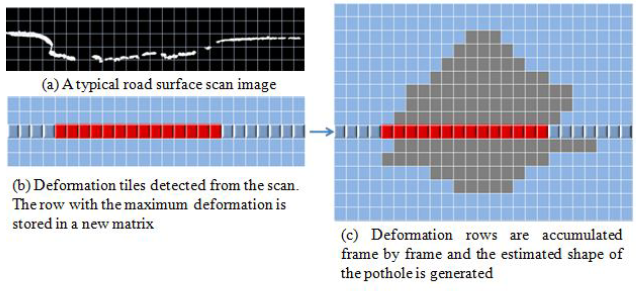
\includegraphics[height=6cm]{Yu2011}
	\caption[Matriz de deteção de um buraco]{Matriz de deteção de um buraco \footnotemark}
	\label{fig:sensor_kinect}
\end{figure}
\footnotetext{\cite{Yu2011}}

Já em \cite{He2011} as linhas vermelhas projetadas no solo são provenientes de uma luz \emph{led} de baixa potência, também perpendiculares à estrada. Este sistema utiliza duas câmeras para fazer a deteção da linha, aumentando a precisão no que toca à classificação do buraco quanto à sua profundidade.
De modo a diminuir ruído existente na imagem, é utilizado o método de Otsu para deteção da linha, bem como uma avaliação dos \emph{pixeis} da vizinhança para que possam ser eliminados falsas deteções, uma vez que a linha é composta por vários \emph{pixeis} de cor semelhante.
Por fim a coloração da imagem é invertida, e é feita uma dilatação e uma contração para uma melhor definição da linha detetada.
Este sistema consegue apresentar erros inferiores a 2mm em termos de profundidade quando comparado com instrumentação de alta precisão para medição de irregularidades.

\begin{figure}[htbp]
	\centering
	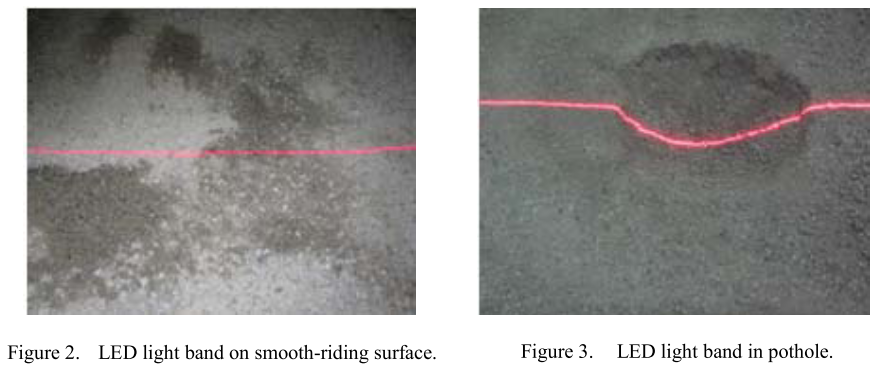
\includegraphics[height=4.4cm]{He2011}
	\caption[Comparação da linha em superfície lisa e num buraco]{Comparação da linha em superfície lisa e num buraco \footnotemark}
	\label{fig:sensor_kinect}
\end{figure}
\footnotetext{\cite{He2011}}
\vspace{5cm}

\subsection{Sensor ultrassónico}
\label{subsec:sensor_ultrassonico}
Outra abordagem completamente diferente é a utilização de sensores ultrassom.
Um sensor ultrassónico é um dispositivo utilizado para medir a distância a um objeto que utiliza ondas sonoras. Este dispositivo mede a distância enviando uma onda sonora com uma frequência específica e aguarda que a onda sonora retorne.
Ao gravar o tempo decorrido entre emissão da onda sonora e a onda sonora de retorno, é possível calcular a distância entre o sensor e o objeto.
Uma vez que se sabe que o som viaja através do ar a cerca de 344m/s, é possível multiplicar o tempo de viagem da onda sonora por 344 metros para encontrar a distância total da viagem da onda sonora, sendo que este valor representa a distância de ida e volta da onda pelo que para encontrar a distância até o objeto, basta dividir esta distância por dois.
Esta é uma opção semelhante à que foi tomada neste projeto na medida em que é quase obrigatório passar por um buraco para fazer a sua deteção, ao contrário da análise de imagens em que é possível evitá-los. 
Em \cite{Hegde2015} é mostrado um protótipo que permite a deteção de buracos através de um sensor ultrassónico testado num protótipo autónomo que comunica com outro veículo de modo a ambos ajustarem as suas velocidades dependendo da qualidade da estrada, diminuindo-a sempre que são detetados buracos.
Para a comunicação foi utilizado um módulo ZigBee que permite estender a comunicação a mais veículos em trabalhos futuros.
O sistema apresentou bons resultados em estradas simuladas mas foi necessário fazer uma calibração específica para este protótipo, sendo que é referido nas conclusões a necessidade de um ajuste aos valores de deteção, consoante o veículo onde o sistema se encontra montado.
Este fator é um grande inconveniente pois depende de cada veículo e da qualidade das suspensões pois caso a suspensão seja muito sensível poderão ser detetados falsos positivos.
\cite{Madli2015} é um projeto mais elaborado, em que uma montagem semelhante é utilizada num veículo e o conceito é testado em estradas reais.
Este sistema tem também a vantagem de detetar elevações no asfalto, através de uma diminuição da distância entre o sensor e o asfalto, ao contrário do que acontece num buraco em que a distância aumenta.
O sistema é também composto por um módulo GPS e outro GSM para que seja possível determinar as coordenadas de uma deteção e enviá-las para um telemóvel, através de uma mensagem de texto, onde é possível consultar e armazenas todas as deteções.
Foi também desenvolvida uma aplicação Android que determina a localização do utilizador e, caso a distância até uma deteção anterior seja inferior a 100m, um alerta é gerado para que o utilizador possa ajustar a sua velocidade em relação às condições do asfalto.
Apesar dos bons resultados na deteção, o sistema tem algumas falhas ao nível da comunicação com o utilizador pois não é possível remover deteções no caso delas serem reparadas, sendo enviados avisos mesmo que uma estrada se encontre em boas condições.
Também existe o mesmo problema que em \cite{Hegde2015} quando avaliada a instalação do sistema. Uma vez que este não se encontra no quadro do veículo, o sistema pode detetar falsos positivos devido a oscilações no terreno que não sejam causadas por buracos nem lombas mas apenas pelo asfalto defeituoso.

\begin{figure}[hbtp]
	\centering
	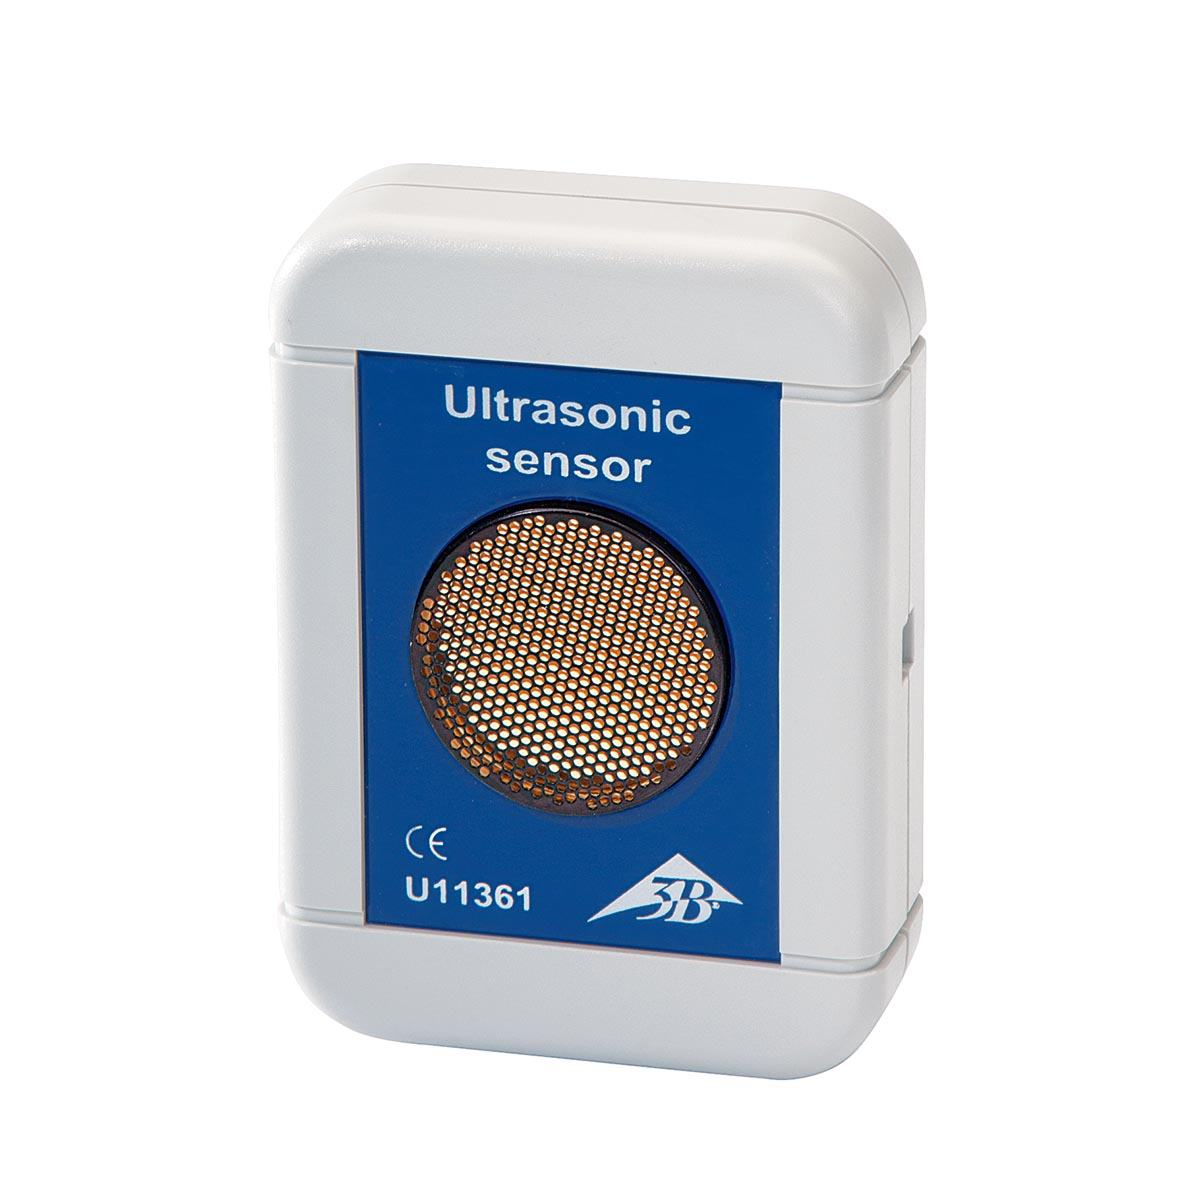
\includegraphics[height=6cm]{ultrassom}
	\caption{Sensor Ultrassom}
	\label{fig:sensor_ultrassom}
\end{figure}

\subsection{Acelerómetro}
\label{subsec: acelerometro}
Esta será a abordagem a ser utilizada e aquela em que os artigos analisados se mostram mais relevantes, devido à semelhança com o projeto que se pretende desenvolver. Em \cite{Mednis2011} é utilizado o acelerómetro do telefone e são apresentados vários algoritmos para a determinação do que é ou não um buraco na estrada. São também feitas algumas comparações sobre os resultados que diferentes telefones apresentam, dependendo do seu acelerómetro, tendo em conta a frequência de amostragem e o desvio padrão do eixo Z.
Neste trabalho foi concluído que diferentes telemóveis recolhem diferentes informações no mesmo percurso, sendo crítico que o acelerómetro não esteja incluído no telemóvel para que exista consistência nos dados recolhidos por diferentes utilizadores.
Foram também avaliados quatro métodos de análise de aceleração para determinar deteções de buracos, sendo que o método \emph{"Z-DIFF"} foi o que apresentou melhores resultados.
Graças a esta análise, foi desenvolvido código que pudesse fazer uma análise semelhante à proposta neste trabalho pois este método apresentou resultados positivos em 92\% dos casos.
No que diz respeito a \cite{Fouad}, é um documento semelhante ao anterior mas adiciona um giroscópio para melhor deteção de buracos. Embora os resultados apresentados sejam bons, terá que ser tido em conta o processamento extra necessário para a utilização dos dados do giroscópio que não parece adicionar muito mais sensibilidade ao sistema.
Neste trabalho, foi também desenvolvida uma aplicação em Android para que os dados recolhidos possam ser armazenados e consultados pelos utilizadores, apesar de não existie comunicação com outros elementos, como uma base de dados para cruzamento de dados com outros utilizadores.
Tal como mencionado nas conclusões, este trabalho não apresentou resultados promissores uma vez que teve uma taxa de sucesso de apenas 75\% graças à utilização do acelerómetro do telemóvel.
Em \cite{Chen2011} foi criado um elemento que contém GPS e acelerómetro e ainda um microprocessador para processar os dados adquiridos. É um sistema muito bem construido e que apresenta vários resultados em estradas de diferentes condições mas poderá ser mais caro do que o pretendido desenvolver neste projeto. No artigo apresentado em \cite{Jang} é apresentada a comunicação entre vários veículos quanto à sua deteção de buracos. Esta ideia é bastante interessante uma vez que possibilita a comunicação em tempo real e caminha na direção das \emph{Smart Cities} e da IoT (Internet of Things - Internet das Coisas em Português).
O sistema é composto por um par de acelerómetros instalado no \emph{tablier} do automóvel e uma antena GPS no seu exterior para a obtenção de coordenadas.
O sistema apresenta resultados bastante precisos mas tem um elevado nível de processamento, pelo que foi necessário um processador mais potente para a gestão dos dados detetados, levando a que o preço total da montagem fosse mais elevado do que o desejado. 
Por fim, é ainda de salientar o trabalho em \cite{Kattan2014} que apresenta uma metodologia semelhante à que foi tomada neste trabalho no que diz respeito à comunicação com uma base de dados mas com pouco desenvolvimento e uma curta fase de testes, sendo que as deteções de buracos tiveram uma taxa de sucesso de apenas 61\% devido à colocação do telemóvel no \emph{tablier} do veículo e à baixa qualidade do algoritmo de deteção.
Foi também utilizado o GPS do telemóvel que apresentou algumas falhas devido à sua baixa precisão e potência, sendo que em alguns casos não era possível obter a localização do utilizador.
Ainda assim é mencionado que para trabalho futuro é proposto um melhoramento deste algoritmo bem como uma nova solução para a deteção de coordenadas.

\begin{figure}[hbtp]
	\centering
	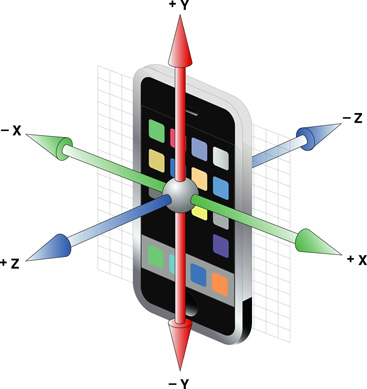
\includegraphics[height=4.5cm]{eixos_acelerometro}
	\caption{Direção dos eixos de um acelerómetro}
	\label{fig:direcao_dos_eixos_de_um_acelerometro}
\end{figure}

\section{Comparação de resultados} % (fold)
\label{sec:comapracao_de_resultados}

Comparando todos os artigos apresentados, é de notar que cada um tem os seus pontos fortes e fracos, como seria de esperar. Para o trabalho que será desenvolvido as qualidades mais importantes a ter em conta são o preço do material utilizado e também o tempo de processamento que o método consome. A tabela \ref{tab:comparacao_de_resultados_de_artigos} mostra as características que serão tidas em conta bem como quais as metodologias que as apresentam.

\begin{table}[htb]
\centering
\caption{Comparação de resultados de artigos}
\label{tab:comparacao_de_resultados_de_artigos}
\begin{tabular}{lcccc}
\multicolumn{1}{c}{} & \begin{tabular}[c]{@{}c@{}}Qualidade de \\ resultados\end{tabular} & \begin{tabular} [c] {@{}c@{}}Preço de \\ material \end{tabular} & \begin{tabular}[c]{@{}c@{}}Tempo de \\ processamento\end{tabular} & \begin{tabular}[c]{@{}c@{}}Processador \\ já incluído\end{tabular} \\
Camera vídeo & \cmark & \xmark & \xmark & \xmark \\
Camera + iluminação & \cmark& \xmark & \xmark & \xmark \\
Ultrassom & \cmark & \cmark & \cmark & \xmark \\
Acelerómetro & \cmark & \cmark & \cmark & \cmark
\end{tabular}
\end{table}

Desta forma, a utilização de um acelerómetro é a mais indicada. Dentro desta metodologia, ainda é possível fazer uma comparação dos vários artigos analisados e tirar algumas conclusões, apresentadas na tabela \ref{tab:comparacao_de_resultados_com_utilizacao_de_acelerometro}.

\begin{table}[htb]
\centering
\caption{Comparação de resultados com utilização de acelerómetro}
\label{tab:comparacao_de_resultados_com_utilizacao_de_acelerometro}
\begin{tabular}{lccccc}
\multicolumn{1}{c}{} & \begin{tabular}[c]{@{}c@{}}Acelerómetro\\ do telefone\end{tabular} & \begin{tabular}[c]{@{}c@{}}GPS do\\ telefone\end{tabular} & \begin{tabular}[c]{@{}c@{}}Giroscópio\\ do telefone\end{tabular} & \begin{tabular}[c]{@{}c@{}}Processador\\ do telefone\end{tabular} & \begin{tabular}[c]{@{}c@{}}Custos além\\ do telefone\end{tabular} \\
{\cite{Mednis2011}} & \cmark & \cmark & \xmark & \cmark & \xmark                              \\
{\cite{Fouad}} & \cmark & \cmark & \cmark & \cmark & \xmark                              \\
{\cite{Chen2011}} & \xmark & \xmark & \xmark & \xmark & \cmark
\end{tabular}
\end{table}

Embora os resultados dos trabalhos em que todos os componentes fazem parte do telefone sejam mais promissores em termos do preço dos materiais, a sua viabilidade é mais baixa, uma vez que um sistema que seja para o público em geral necessita de apresentar resultados consistentes, independentemente da situação e se o acelerómetro não estiver sempre no mesmo sítio (neste caso, o telefone) as leituras de cada irregularidade detetada são alteradas a cada passagem, dependendo do local em que o telefone se encontra, seja no bolso do casaco, no banco do veículo ou no seu \emph{tablier}.
A utilização de GPS é obrigatória para que os buracos detetados possam ser localizados, sendo que um GPS externo pode apresentar mais precisão do que o integrado no telemóvel e evita falhas de receção tal como é referido em \cite{Kattan2014}.
Desta forma, a solução apresentada neste projeto conta com um smartphone do utilizador, bem como um acelerómetro e GPS externos que estão fixados no veículo.
O acelerómetro está colocado diretamente no quadro do veículo de testes de modo a que a qualidade das suspensões não interfira com as leituras.
O GPS foi colocado no interior do veículo pois a sua antena é bastante potente, fazendo com que não seja necessário um local muito específico para a sua colocação.